\section{Results}
\label{sec:results}
\emph{Note that measurements for the Generalized RRR with arity 16 are missing, 
since the experiments took too long due to paging. This supports our third 
hypothesis, but there may be ways to overcome this, as detailed in Section 
\ref{sec:future}.}

\emph{Also Note that the Uncompressed Wavelet Tree timings have been plotted on 
a different graph due to the difference in scale.}\\

\begin{table}[h]
\begin{center}
\begin{tabular}{crr}
\toprule
Arity & \multicolumn{1}{c}{Max Total Classes} &
\multicolumn{1}{c}{Max Total Permutations}\\
\midrule
2 & 16 & 32 768\\
4 & 816 & 1 073 741 824\\
8 & 17 0544 & 35 184 372 088 832\\
\bottomrule
\end{tabular}
\caption{Maximum Total Classes and Offsets possible with a blocksize of 15 for arity 
    values 2, 4, and 8.}
\label{tab:maxclass}
\end{center}
\end{table}


From Figure \ref{fig:unique} we can see how the number of unique classes and 
block permutations increases depending on file size and arity. Table 
\ref{tab:maxclass} shows the maximum of each of these values, and Figure 
\ref{fig:sparse} plots the number of unique classes and block permutations as
a percentage of the values in Table \ref{tab:maxclass}.

Figure \ref{fig:sparse} indicates that in all data sets, around $100$ percent of
the classes and block permutations were encountered for arity 2. In most data
sets, all classes were encountered for arity 4 as well, with the exception being 
DNA, which encountered around $30$ percent.

Figure \ref{fig:unique} shows that the proteins data set had significantly more
unique block permutations than any other data set, while the words data set is 
the only one to have encountered all classes for arity 8. This is because 
protein data is essentially random, so its BWT will not contain long runs of the 
same symbol, reducing the skew of its classes.

\begin{figure}[h]
\begin{center}
$\begin{array}{cc}
\mbox{English} & \mbox{Words} \\
\includegraphics[width=2.5in]{experiments/unique_english} &
\includegraphics[width=2.5in]{experiments/unique_english_ints} \\ \\ \\
\mbox{DNA} & \mbox{Proteins} \\ 
\includegraphics[width=2.5in]{experiments/unique_dna} &
\includegraphics[width=2.5in]{experiments/unique_proteins} \\ \\ \\
\mbox{Sources} & \mbox{XML} \\
\includegraphics[width=2.5in]{experiments/unique_sources} &
\includegraphics[width=2.5in]{experiments/unique_dblp_xml}
\end{array}$
\end{center}
\caption{Number of unique classes and block permutations for each data 
file. The vertical axis represents the total number of classes and block
permutations that were witnessed for the given file size and arity when using 
the Multiary Wavelet Tree with Generalised RRR.}
\label{fig:unique}
\end{figure}
	
\begin{figure}[h]
\begin{center}
$\begin{array}{cc}
\mbox{English} & \mbox{Words} \\
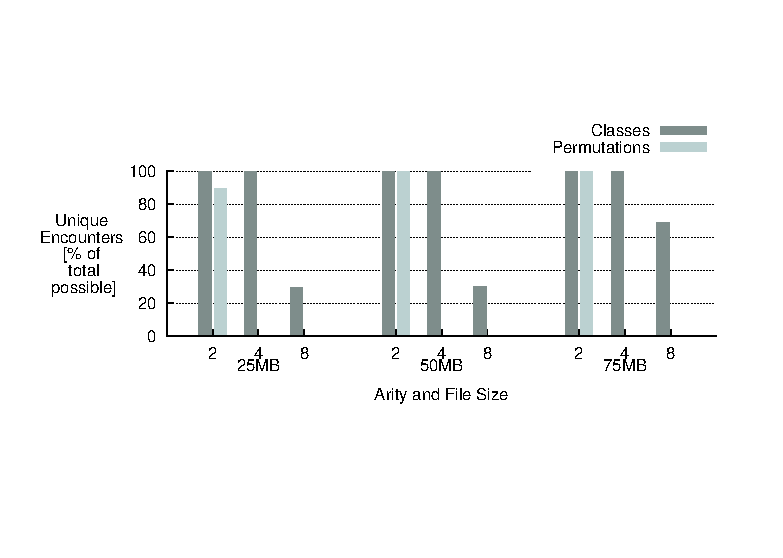
\includegraphics[width=2.5in]{experiments/sparse_english} &
\includegraphics[width=2.5in]{experiments/sparse_english_ints} \\ \\ \\
\mbox{DNA} & \mbox{Proteins} \\ 
\includegraphics[width=2.5in]{experiments/sparse_dna} &
\includegraphics[width=2.5in]{experiments/sparse_proteins} \\ \\ \\
\mbox{Sources} & \mbox{XML} \\
\includegraphics[width=2.5in]{experiments/sparse_sources} &
\includegraphics[width=2.5in]{experiments/sparse_dblp_xml}
\end{array}$
\end{center}
\caption{Sparsity measurements for each data file. The vertical axis represents
the percentage of \emph{total possible} classes and block permutations that were
witnessed for the given file size and arity when using the 
Multiary Wavelet Tree with Generalised RRR. Note that some bars are too small to 
see.}
\label{fig:sparse}
\end{figure}

\clearpage
		\DefFig[Uncompressed Multiary Wavelet Tree
			query times for English files]
			{fig:stime-eng}{experiments/simple_time_english}{0.9}
			{Query times for Uncompressed Multiary Wavelet Tree 
			of increasing arity for each \emph{English} file.}
		
		\DefFig[RRR Wavelet Tree query times for 75MB English file]
			{fig:time-eng-75}{experiments/time_english_75MB}{0.9}
			{Query times for RRR Wavelet Trees of increasing arity
			for the 75MB \emph{English} file.}
	
			\begin{figure}[h]
			\begin{center}
			$\begin{array}{cc}
			\mbox{(25MB English file)} & 
			\mbox{(50MB English file)} \\
			\includegraphics[width=2.5in]{experiments/time_english_25MB} &
			\includegraphics[width=2.5in]{experiments/time_english_50MB}
			\end{array}$
			\end{center}
			\caption{Query times for RRR Wavelet Trees of increasing arity
			for the 25MB and 50MB \emph{English} files.}
			\label{fig:time-eng-25-50}
			\end{figure}
			
From Figure \ref{fig:stime-eng} we can see how increasing the arity affects
querying an uncompressed Wavelet Tree. It is slower for increasing file size
because it is calculating rank queries without the assistance of RRR.

From Figures \ref{fig:time-eng-75} and \ref{fig:time-eng-25-50} we are able 
to see that increasing the file size does not significantly affect the time
performance of the Wavelet Trees which utilise RRR.

The Generalised RRR is slower than Claude's. We suspect that this is due to our 
use of pointers, as required to create a sparse table, whereas Claude's avoids 
dereferencing and may make better use of cache. The trend is similar to the
other Multiary Wavelet Trees, though.

The Multi-Binary RRR Wavelet Tree is faster than Claude's when the arity is 
increased. It is slower at arity 2 possibly due to optimisations in Claude's
Wavelet Tree code, or because we need to do an extra calculation to work out
the binary rank of all previous symbols (see Section 
\ref{sec:multi-bin-rrr}).

\clearpage
		\DefFig[Memory consumption for 75MB English file]
			{fig:mem-eng-75}{experiments/mem_english_75MB}{0.9}
			{Memory consumption for Wavelet Trees of increasing arity for
			the 75MB \emph{English} file. 
			The memory required for each data structure is the size coefficient 
			multiplied by the original file size.
			The bar stacked on top is the space for
			the supporting RRR count table. The bar underneath is the space for
			the shape of the Wavelet Tree (which had negligible overhead) and 
			each of its
			nodes, as RRR sequences or not. The Uncompressed Wavelet Tree is
			the only one which does not have a RRR count table.}
		
Figure \ref{fig:mem-eng-75} shows the memory consumption of the structures for 
each English file. As the smaller sized files have similar size coefficients, we
only show the graphs for the 75MB files.

Note that even though the Generalised RRR Wavelet Tree size (which 
includes the RRR sequences it stores) is smaller than the original text, and 
smaller than the Multi-Binary RRR Wavelet Tree, the size to contain the 
supporting RRR count structure is large.

		\DefFig[Memory consumption for 75MB Words file]
			{fig:mem-words-75}{experiments/mem_english_ints_75MB}{0.9}
			{Memory consumption for Wavelet Trees of increasing arity for
			the 75MB \emph{Words} file. The memory required for each data 
			structure is the size coefficient 
			multiplied by the original file size.
			The bar stacked on top is the space for
			the supporting RRR count table. The bar underneath is the space for
			the shape of the Wavelet Tree (which had negligible overhead) and 
			each of its
			nodes, as RRR sequences or not. The Uncompressed Wavelet Tree is
			the only one which does not have a RRR count table.}

		\DefFig[Memory consumption for 75MB Proteins file]
			{fig:mem-prot-75}{experiments/mem_proteins_75MB}{0.9}
			{Memory consumption for Wavelet Trees of increasing arity for
			the 75MB \emph{Proteins} file. The memory required for each data 
			structure is the size coefficient 
			multiplied by the original file size.
			The bar stacked on top is the space for
			the supporting RRR count table. The bar underneath is the space for
			the shape of the Wavelet Tree (which had negligible overhead) and 
			each of its
			nodes, as RRR sequences or not. The Uncompressed Wavelet Tree is
			the only one which does not have a RRR count table.}
		
		\DefFig[Memory-Time tradeoff for 75MB English file]
			{fig:tradeoff-eng-75}{experiments/tradeoff_english_75MB}{0.8}
			{Memory-Time tradeoff for RRR Wavelet Trees of increasing arity for
			the 75MB \emph{English} file. The memory required for each data 
			structure is the size coefficient 
			multiplied by the original file size.}
		
		\DefFig[Memory-Time tradeoff for 75MB Words file]
			{fig:tradeoff-words-75}{experiments/tradeoff_english_ints_75MB}{0.8}
			{Memory-Time tradeoff for RRR Wavelet Trees of increasing arity for
			the 75MB \emph{Words} file. The memory required for each data 
			structure is the size coefficient 
			multiplied by the original file size.}
		
		\DefFig[Memory-Time tradeoff for 75MB Proteins file]
			{fig:tradeoff-prot-75}{experiments/tradeoff_proteins_75MB}{0.8}
			{Memory-Time tradeoff for RRR Wavelet Trees of increasing arity for
			the 75MB \emph{Proteins} file. The memory required for each data 
			structure is the size coefficient 
			multiplied by the original file size.}
		
The Proteins files have less classes (Figure \ref{fig:sparse}) but more 
permutations (Figure \ref{fig:unique}) than the Words files. This may be the 
cause of the large table size for the Generalised RRR Wavelet Tree in Figure
\ref{fig:mem-prot-75} compared with that of the Words file in Figure 
\ref{fig:mem-words-75}.

In all cases, the Generalised RRR Wavelet Tree size is less than the original
text size. It is important to note that the RRR count table can be shared among
Wavelet Trees, but this may cause it to grow to its full amount, depending on
the distribution of classes for the type of text we are indexing, as more 
classes and permutations may be encountered.

The tradeoff between memory and query time for the English files can be seen in 
Figure \ref{fig:tradeoff-eng-75}. All other test data follows a similar trend, 
so the graphs have been omitted\footnote{The 
other graphs are available at http://github.com/alexbowe/honours-thesis/.}, with 
the exception of Words (Figure 
\ref{fig:tradeoff-words-75}), Proteins (Figure \ref{fig:tradeoff-prot-75}) and
DNA.

In Figure \ref{fig:tradeoff-words-75} The Generalised RRR Wavelet Trees queries 
slow down for arity 8. This may be due to fragmentation of the RRR count table
memory; as the Wavelet Tree becomes less shallow as its arity increases, the
benefit of cache may also diminish, since the RRR count table will become
larger and possibly dispersed throughout memory. This would not affect the other
RRR Wavelet Trees as their RRR count tables are contiguous and small, making 
the better use of cache.

Figure \ref{fig:tradeoff-prot-75} shows the query time increasing slightly for 
arity 4, then decreasing again for arity 8. This may be due to the small 
alphabet size of the Proteins file, meaning the Wavelet Tree would not get much 
shallower, and as above the performance may be dominated by cache. This trend 
was seen in DNA as well, which also has a small alphabet.
